\documentclass[11pt,a4paper,oneside]{report}

% Packages
\usepackage[utf8]{inputenc}		
\usepackage[T1]{fontenc}			
\usepackage[english]{babel}						% Speling Errors? Me? Never!

\usepackage{amsmath}							% For all your math needs...
\usepackage{amsfonts}							% ...and beyond...
\usepackage{amssymb}							% ...and even further.
\usepackage{makeidx}							% We have a number of indexes.
\usepackage{url}								% URLs in bib
\usepackage{graphicx}							% For pictures and stuff.
\usepackage[pdfusetitle]{hyperref}				% Not really necessary.
\usepackage[acronyms,nohypertypes={acronym,main},nopostdot]{glossaries} % For the glossary.
\usepackage[bottom,perpage,multiple]{footmisc}	% Place footnotes at the bottom of the page, restart counting each page and merge multiple footnotes.
\usepackage{csquotes}							% Quoting. Probably only used in the glossary.
\usepackage[strings]{underscore}				% Bibtex is confused by underscores in URLs. Yeah... underscores.
\usepackage{censor}								% For ████ing that ████ed piece of ████. Actually only for development.
\usepackage{listings}							% Code Snippets.
\usepackage{color}								% Colorful code snippets :3
\usepackage[singlelinecheck=off]{caption}		% Make captions left aligned even if single line.
\usepackage{tocbibind}							% Include ToC in ToC.
\usepackage{nameref}


% Dev Only
\usepackage{marginnote}							% For development comments.
\renewcommand*{\marginfont}{\tiny}
\usepackage[marginparsep=3mm, marginparwidth=2cm]{geometry}

% Disable Marginnotes:
%\renewcommand*{\marginnote}[1]{}

% Glossary Styling
\setacronymstyle{short-long}
\setglossarystyle{altlist}
\makenoidxglossaries{}
\glstoctrue{}

% Listings Styling
\definecolor{grey}{rgb}{0.8,0.8,0.8}
\lstset{
	tabsize=2,
	rulecolor=\color{black},
	numberstyle=\color{grey},
	numbersep=10pt,
	framesep=5pt,
	xleftmargin=5pt,
	xrightmargin=5pt,
	numbers=left,
	escapeinside={(*@}{@*)},
	keepspaces=true,
	frame=shadowbox,
	captionpos=b,
	breaklines=false,
	basicstyle=\ttfamily\footnotesize,
	aboveskip=20pt,
	belowskip=10pt,
	keywordstyle=\color{blue}\ttfamily,
	stringstyle=\color{green}\ttfamily
}
\lstdefinestyle{YAML}{
	morekeywords={FROM,COPY,ENTRYPOINT,ADD,CMD,HEALTHCHECK,RUN}
}


% Header Imports
\graphicspath{{img/}}
\bibliographystyle{alpha}

\def\A{{\mathcal{A}}}
\def\B{{\mathcal{B}}}
\def\C{{\mathcal{C}}}
\def\D{{\mathcal{D}}}
\def\E{{\mathcal{E}}}
\def\F{{\mathcal{F}}}
\def\G{{\mathcal{G}}}
\def\H{{\mathcal{H}}}
\def\I{{\mathcal{I}}}
\def\K{{\mathcal{K}}}
\def\L{{\mathcal{L}}}
\def\M{{\mathcal{M}}}
\def\N{{\mathcal{N}}}
\def\O{{\mathcal{O}}}
\def\P{{\mathcal{P}}}
\def\Q{{\mathcal{Q}}}
\def\R{{\mathcal{R}}}
\def\S{{\mathcal{S}}}
\def\T{{\mathcal{T}}}
\def\U{{\mathcal{U}}}
\def\V{{\mathcal{V}}}
\def\W{{\mathcal{W}}}
\def\X{{\mathcal{X}}}
\def\Y{{\mathcal{Y}}}
\def\Z{{\mathcal{Z}}}

\def\AA{{\mathbb{A}}}
\def\BB{{\mathbb{B}}}
\def\CC{{\mathbb{C}}}
\def\DD{{\mathbb{D}}}
\def\EE{{\mathbb{E}}}
\def\FF{{\mathbb{F}}}
\def\GG{{\mathbb{G}}}
\def\HH{{\mathbb{H}}}
\def\II{{\mathbb{I}}}
\def\KK{{\mathbb{K}}}
\def\LL{{\mathbb{L}}}
\def\MM{{\mathbb{M}}}
\def\NN{{\mathbb{N}}}
\def\OO{{\mathbb{O}}}
\def\PP{{\mathbb{P}}}
\def\QQ{{\mathbb{Q}}}
\def\RR{{\mathbb{R}}}
\def\SS{{\mathbb{S}}}
\def\TT{{\mathbb{T}}}
\def\UU{{\mathbb{U}}}
\def\VV{{\mathbb{V}}}
\def\WW{{\mathbb{W}}}
\def\XX{{\mathbb{X}}}
\def\YY{{\mathbb{Y}}}
\def\ZZ{{\mathbb{Z}}}
\def\\{{\setminus}}

\newcommand{\footurl}[2]{\footnote{\url{#1}, last accessed on #2.}}
% Glossary

% #1: Id (uima)
% #2: Shortname (UIMA)
% #3: Longname (Unstructured Information Management Applications)
% #4: Description (UIMA are software systems that...)
\newcommand{\newacr}[4]{\newglossaryentry{glos:#1}{name={#3},description={#4}} \newacronym{acr:#1}{#2}{\gls{glos:#1}} }

\newacr{uima}{UIMA}{Unstructured Information Management Applications}{UIMA are software systems that analyze large volumes of unstructured information in order to discover knowledge that is relevant to an end user. An example UIM application might ingest plain text and identify entities, such as persons, places, organizations; or relations, such as works-for or located-at.}

\newcommand{\uima}{\gls{acr:uima}}

\newglossaryentry{glos:dkpro}{%
    name=DKPro,
    description={DKPro is a community of projects focussing on re-usable Natural Language Processing software}
    }

\newcommand{\dkpro}{\gls{glos:dkpro}}


% Meta Data Definitions
\newcommand{\authortext}{Simon Gehring}
\newcommand{\street}{Am Jesuitenhof}
\newcommand{\email}{gehring@uni-bonn.de}
\newcommand{\housenumber}{3}
\newcommand{\postal}{53117}
\newcommand{\city}{Bonn}
\newcommand{\mn}{2553262}

\newcommand{\doctype}{Master Thesis}
\newcommand{\titletext}{Scaling UIMA}
\newcommand{\subtitletext}{} % Don't know anything interesting.
\newcommand{\field}{Computer Science}
\newcommand{\organization}{Rheinische Friedrich-Wilhelms-Universität Bonn}
\newcommand{\cooperation}{Fraunhofer-Institut für Kommunikation, Informationsverarbeitung und Ergonomie}
\newcommand{\cooperationTwo}{PricewaterhouseCoopers GmbH}

\newcommand{\supervisorOne}{Prof.~Dr.~Heiko \textsc{Röglin}}
\newcommand{\supervisorTwo}{Dr.~Timm \textsc{Heuss}}


% Meta Data Compiling
\title{\titletext}
\author{\authortext}
\date{\today}
\newcommand{\address}{\street{} \housenumber{}\linebreak
\postal{} \city{}}

% Document Start
\begin{document}
%\doctype Master Thesis
%\titletext Some Title
%\subtitletext Some Subtitle
%\field Computer Science
%\organization Rheinische Friedrich-Wilhelms-Universität Bonn
%\cooperation Fraunhofer-Institut für Kommunikation, Informationsverarbeitung und Ergonomie
%\address

\begin{titlepage}    
    \centering
	{\scshape\Large \doctype{}\par}
	{\scshape\large \field{}\par}
	\vspace{1.5cm}
	{\Huge\bfseries \titletext{}\par}
	\vspace{1cm}
	{\LARGE \subtitletext{}\par}
	\vspace{2cm}
	{\Large\itshape \authortext{}\par}
	\vspace{0.35cm}
	{\large \address\par}
	{\large \email\par}
	{\large Matriculation Number \mn\par}
	\vfill
	    { At the \par}
	    \vspace{0.1cm}
	    {\scshape\large\organization{}\par}
	    \vspace{0.1cm}

%{in cooperation with the\par}
%    \vspace{0.1cm}
%    {\scshape\large\cooperation{}\par}	
%    \vspace{0.1cm}
%    {and\par}
%    \vspace{0.1cm}
%    {\scshape\large\cooperationTwo{}\par}
	\vfill	
	supervised by\par
	\supervisorOne{} and 
	\supervisorTwo{}
	

	

	\vfill

% Bottom of the page
	{\large \today\par}
\end{titlepage}
\pagenumbering{roman}
\tableofcontents{}
\newpage{}
\setcounter{page}{1}
\pagenumbering{arabic}

% Precontent
\begin{abstract}
In this thesis, we will evaluate different means of scaling \uima{}, using modern technologies like \docker{}, a container virtualization solution, and \spark{}, a cluster computing framework. \marginnote{Update, was wir eigentlich evaluaten, sobald das Evaluation chapter fertig ist.}We will compare said implementations with the native \uimaas{} approach in terms of processor and memory efficiency, ease of implementation and maintainability. The evaluation will be based on a specific scenario, however it will be easily configurable by exchanging very few lines of code. 

\end{abstract}

% Content
% !TeX root = ../Main.tex

\chapter{Introduction}



\section{Motivation}
Idee: NLP benötigt große Daten, was im Grunde BigData ist (Größenordnung Peta oder Exabyte.)
Muss entsprechend skaliert werden. Das geht einzeln mit verschiedenen NLP Frameworks, aber UIMA
ist halt UIMA und generisch. Wär also geil wenn das anständig skalierbar ist.
Daten von Statista finden, eventuell sogar Graphen eventuell sogar Unternehmensdaten(?)

Weiterhin Name-Dropping von Watson. Was ist GATE oder spaCy

\section{Implementation Requirements}
Welche Kriterien für die Skalierung werden überprüft und warum ist das sinnvoll?



\section{Outline}
Ich outline hier halt die gesamte restliche Thesis. Im Großen und Ganzen ist das hier nur ein unvollständiges und glorifiziertes Inhaltsverzeichnis. 		% Einführung, Motivation, Related Work
% !TeX root = ../Main.tex

\chapter{Basics}
\label{ch:basics}
In this chapter, the two most important technologies for the framework are explained. This is necessary to get an understanding of the technical difficulties it challenges and how it works. First, in Section~\ref{sec:uima} \uima{} is introduced. After an in-depth introduction into the original framework designed by IBM, \uimafit{} will be explained. \uimafit{} builds on top of \uima{}, providing the developer with a native Java interface for creating and instantiating plug-ins. Strongly related to the framework introduced in Chapter~\ref{ch:implementation} are the two native scaling frameworks \uimacpe{} and \uimaas{}. 

\marginnote{Ich habe es zwar nicht benutzt, aber eine kleine Einführung in HDFS könnte nützlich sein. Ich werde häufiger (im Kontext von BigData) anmerken, dass Daten vermutlich von einem verteiltem Dateisystem, etwa einem HDFS kommen und dahin geschrieben werden.}

The second section of this chapter will be about \spark{}. While no advanced knowledge is needed to comprehend the usage of \spark{} as a distributed computation framework, it will still be a substantial part of the \uima{} scaling framework in Chapter~\ref{ch:implementation}. Thus, a rather superficial overview of its structure and distribution algorithm will be given.

Since numerous attempts have been made, scaling \uima{} in different settings, with varying implementation requirements, some related work will be presented in Section~\ref{sec:related}, namely Leo, providing a native Java interface for \uimaas{}, and v3NLP, a framework especially designed for usage in a medical environment and with plug-ins of such sort.

Although most important aspects and concepts of \uima{} are also defined in the specifications, some minor changes and additions were made in the implementations. Since the framework must handle the actual implementation, all the presented concepts will be taken from Apache \uima{} instead of the \uima{} specification of 2009.



\section{UIMA-Family}
\label{sec:uima}
Unstructured Information Management Architecture (UIMA) Version 1.0 itself is an \oasis{} standard from 2009\footurl{http://docs.oasis-open.org/uima/v1.0/uima-v1.0.html}{2018-09-03} that defines an interface for software components, or plug-ins, which are called analytics. Those analytics are supposed to analyze unstructured information and assign machine readable semantics to it. The standard also defines ways to represent and interchange this data between analytics in favor of interoperability and platform-independence. 

Apache \uima{} is the open-source implementation of said \uima{} specification. A common problem with Apache \uima{} is scaling \cite{divita2015scaling,epstein2012making,ramakrishnan2010building}. It  provides two distinct interfaces to analyze larger collections of unstructured data itself, with one being \uimaas{} and the other being the more dated and less flexible \cpe{} \cite{OASIS:UIMA:2009}.
Apache \uima{} is available for Java and C++, while its scaling solutions, \uimacpe{} and \uimaas{} are only available for Java, which is why this thesis focuses on the Java implementation. Since \uima{} and Apache \uima{} have very similar names, which may lead to confusion it is common practice to call the implementation simply \uima{} and explicitly state when talking about the specification. This practice will be adopted for the rest of the thesis.




Unbedingt bilder hinzufügen und establishen was eine Pipeline ist!!1!

\subsection{Apache UIMA}

Apache \uima{} is one of few general approaches to implement \nlp{} solutions and the only commonly known implementation of the specification with the same name. With a very modular architecture, \uima{} is a popular tool that can easily be applied to a majority of \nlp{} problems. A large part of the popularity of \uima{} stems from the large \dkpro{} collection of components, containing hundreds of analysis modules and precomputed language models \cite{eckartdecastilho-gurevych:2014:OIAF4HLT}, which are easily imported into existing Java projects with the build automation tool Apache Maven \cite{dkpro}.

\uima{} is usually used to process not a single but whole corpora of documents. A document in this sense is text, although the \uima{} specification permits other data types as well. However, \uima{} can not handle other data types without serializing it first. The \uima{} specification, as well as the implementation do not directly pose limitations to the document size but since documents are stored in native Java String variables, which itself are implemented as arrays of chars, the practical limit of documents sizes is dependent on the \jvm{} version and lies around one to two gigabytes \cite{so:javastrings} per document. In the context of \uima{}, such a document is called a \sofa{}.

An analytic in the \uima{} specification is called an \emph{Analysis Engine} in the implementation. For the most part, an \anen{} is code, that gets an input \cas{} and produces a number of analysis results on the \sofa{}. Common examples for \anens{} are Segmentation, Tokenization, and Part-of-Speech finding algorithms \cite{dkpro}. However, since an \anen{} contains arbitrary Java code any form of analysis can be instrumentalized by \uima{}. It is defined by an \xml{} Analysis Engine descriptor. Such an \anen{} can either be a so-called \emph{primitive} or an \emph{aggregate} engine. An aggregate engine simply contains one or more other \anens{}, that are aggregated into one single engine.

Analysis results are stored as annotations. An annotation has at least two attributes \lstinline[language=Java]|int begin| and \lstinline[language=Java]|int end|, indicating the start and end index of the \sofa{}s substring this annotation is associated with. This concept is theoretically extendable to any kind of \sofa{} that contains any sort of subsets, for example images or audio and video streams. However, this is impractical for reasons mentioned above. It is possible, but uncommon, to define other types of subsets on a string that -- for example -- permit multiple segments. Such subsets can be implemented in a custom implementation of the \lstinline|AnnotationBase| class, which in turn may omit the concept of a \lstinline|begin| and \lstinline|end|. Since an important reason of the popularity of \uima{} lies in the large \anen{} repositories and the possibility to reuse already published code, custom annotation implementations are rarely used because it would most likely lead to incompatibilities. However, sub classing the \lstinline|Annotation| class is often done to ensure type safety. Building such an annotation hierarchy leads to the creation of a Type System.

The Type System is a schema of all available types of annotations that may be associated with a current \sofa{}, thus it provides the meta data for the annotations. It is defined by an \xml{} Type System descriptor that is usually used by the \emph{JCasGen}, a Java code generator for \uima{} types. A \xml{} Type System descriptor may define an super Type System from which to inherit all types. This can be used to subclass types that are not defined in the current context and encapsulate all in a single larger Type System.

The \sofa{}, all analysis results in form of annotations that are compliant to an underlying Type System and the Type System itself are stored together in one large object, called a \cas{}. It is the sole input an \anen{} gets, since it incorporates the complete context needed. The annotations are stored in a larger index to optimize for efficient access. Furthermore, a \cas{} object provides different Views, lightweight versions of a \cas{}, that store their own \sofa{} and annotation index. These views are identified by a String, while the original data of the \cas{} is usually called the \emph{Initial View}.

A \emph{Collection Reader} implements an interface very similar to the well-known \lstinline|Iterator|, namely it provides the functions \lstinline|boolean hasNext()| and \lstinline|CAS getNext()|. A Collection Reader usually takes the role of initializing the \cas{} with the \sofa{}. Well known Collection Readers achieve this by reading from a file system, a database or \lstinline|Collection| object, but any other collection may be read by implementing a custom Collection Reader. It is also configured by writing an \xml{} descriptor file.

Multiple Analysis Engines that form a complete flow of analysis are commonly known as a \emph{pipeline}. Since multiple \anens{} can be aggregated into one, a pipeline is usually an instance of a single aggregate analysis engine. Sometimes a pipeline is meant to also include a Collection Reader, however this will not be the case in this thesis. Because of the convention to call analysis results annotations, \anens{} are often called \emph{Annotators}, which is not correct in general, since engines do not need to attach any annotations to the input \cas{}.

\begin{figure}[hbt]
	\centering
	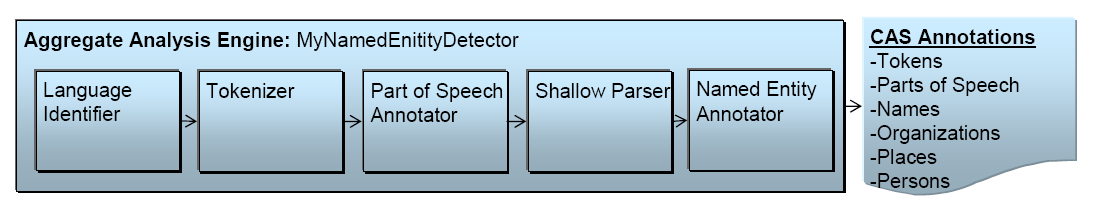
\includegraphics[width=1\textwidth]{uima-pipeline}
	\caption[An example UIMA pipeline for NER.]{An example \uima{} pipeline for named entity recognition \cite{uimasdk}.}
	\label{fig:uimaner}
\end{figure}

Figure~\ref{fig:uimaner} shows a simplified view of an analysis pipeline for named entity recognition. Given a \cas{} by a Collection Reader (omitted here), the pipeline which is really just a aggregate Analysis Engine starts to identify the language of the text with an analysis engine specifically designed to do exactly this. This \anen{} stores the results inside the \cas{} and forwards it to the next engine in line, which is a tokenizer. 

A tokenizer annotates words, sentences and punctuation and is highly language dependent. It uses the analysis result given by the \anen{} before to decide upon an algorithm or model to use according to the found language. After tokenization, a Part-Of-Speech Tagger annotates each words part of speech with a different annotation according to a tag set. There are a number of tag sets for most languages, as for example the Penn Treebank Project tag set\footurl{https://www.ling.upenn.edu/courses/Fall_2003/ling001/penn_treebank_pos.html}{2018-09-08} for English and the \stts{} for German. The Part-Of-Speech Tagger is highly language dependent because of this. It also utilizes the results of the tokenizer, since it iterates over all annotations that are words.

Afterwards the \cas{} gets put into a Shallow Parser, which analyzes Part-Of-Speech tags and their semantic relation among other tags in the same sentence. In a sentence `I like green apples.' a Part-Of-Speech Tagger would correctly decide that `green' is an adjective and apples is a noun. However, a parser would combine those two to form `green apples', a Noun Phrase, because `green' is an adjectival modifier of `apples'. A Parser may also be used to improve the results of a previous Part-Of-Speech tagging.

A Named Entity Recognizer then takes the \cas{} object and looks for fitting entities. This is commonly a Noun of a given list, but can be more sophisticated, depending on the wanted precision, the entity type and computation speed. After the last part of the pipeline returns, the analysis is done. The resulting \cas{} now includes a number of analysis results in form of annotations and can now be extracted or processed further.

\subsection{UIMAfit}
\label{ssec:uimafit}
Since \uima{} needs \xml{} descriptor files to configure and describe most of its components, especially pipelines and type systems, developing for it is very \xml{} heavy and leads to code that is hard to maintain. Apache \uimafit{} is a framework that builds on \uima{}, providing an interface to programmatically describe, instantiate and deploy \uima{} components \cite{ogren-bethard:2009:SETQA-NLP}. \uimafit{} also provides an interface to dynamically write \xml{} descriptor files for \uima{} components. However, since it is able to instantiate and deploy said components without the need of \xml{} files, those are mostly ignored. \uimaas{}, a native \uima{} scaling framework described in Section~\ref{ssec:uimaas}, is known to be widely incompatible with \uimafit{} which is what led to the creation of Leo, described in Section~\ref{ssec:leo}.

\uimafit{} has been part of the Apache \uima{} project since 2012 and is therefore officially supported \cite{github:uimafit}. 



\subsection{UIMA-CPE}
\label{ssec:uimacpe}
\uimacpe{} was the first method to add distributed computation capability to \uima{}. Nowadays it has been replaced by \uimaas{} and is mostly obsolete. It made use of so called \emph{\cas{} Consumers}, engines that do not analyze the \cas{}, but extract the needed analysis results from it and process the data as wanted. Common uses for \cas{} Consumers are writing analysis results into a database or serializing the whole \cas{} into a \xmi{} file. \cas{} Consumers have been deprecated and replaced by \anens{} since 2006 \uimacpe{} because \cas{} Consumers do not provide any new functionality or are semantically different from Analysis Engines. Historically a \cas{} Consumer would not add anything to a \cas{} object. This convention of a reading-only Analysis Engine is often used to provide maximum modularity among \uima{} engines.


Another concept exclusive to \uimacpe{} are \cas{} Initializers, which also have been deprecated for over a decade, but are still included in \uima{}. A \cas{} Initializer was responsible to populate a \cas{} from an object given by the Collection Reader. It therefore implemented the function \lstinline|initializeCas(Object document, CAS cas)|. This was used for more complex collection reading capabilities and \cas{} Initializers are generally seen as a plug-in to Collection Readers to extend their functionality. If -- for example -- only table of contents of larger documents are meant to be analyzed, then a Collection Reader would read the whole document and pass it to the \cas{} Initializer, which would search for a table of contents and fill the \cas{} with its findings and discard the rest of the document.


\begin{figure}[hbt]
	
	\centering
	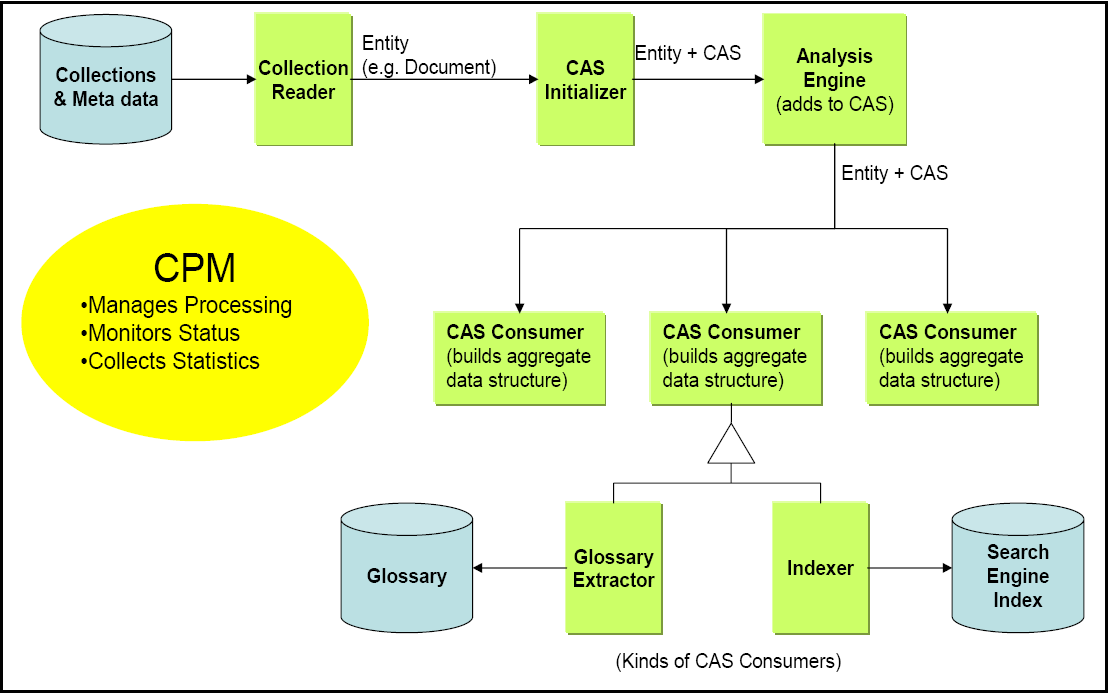
\includegraphics[width=1\textwidth]{uima-cpe}
	\caption[All \uimacpe{} components.]{All \uimacpe{} components \cite{uimacpe}.}
	\label{fig:uimacpe}
\end{figure}


Figure~\ref{fig:uimacpe} shows a complete example pipeline. It starts with any kind of collections, maybe containing meta data. A common example would be a folder hierarchy with last modified timestamps. The Collection Reader is aware of this collection and implements an \lstinline|Iterator| like interface, returning plain \lstinline|Object|s. These are given to the \cas{} Initializer. Notice, that the \cas{} Initializer must be aware of what kind of entity the Collection Reader sends it. The \cas{} Initializer then fills a \cas{} object with some data from the given input \lstinline|Object|. It might also create some first annotations to store meta data inside the \cas{}, such as the source document \URL{} or the creation timestamp. 

The \cas{} is then sent to the pipeline, containing one or more \anens{}, providing analysis results in form of annotations that are stored inside the \cas{}. Notice that the corresponding \cas{} object for a document always stays the same identical object. A \cas{} and its corresponding document are therefore closely associated to each other. After the analysis phase, the \cas{} is sent to the \cas{} Consumers. Those aggregate the analysis results and process it further. This process is commonly the indexing into a database or printing logs to a log file or console. Since \cas{} Consumers have read-only access to the \cas{} object they get, all of them might be processed in parallel, provided that the consumers do not interfere with each other.

All these components in combination with the \uima{} \cpm{} forms the \uimacpe{}. The Collection Processing Manager provides configuration options for deployment, instantiation, and error recovery. It monitors the whole process and collects statistics. By configuration of the \cpm{} scaling is possible either locally or on distributed machines.

For all three components introduced in this Section~\ref{ssec:uimacpe} \xml{} descriptor files are needed for configuration. The concept of a \uimacpe{} is widely incompatible with \uimafit{}, described in Section~\ref{ssec:uimafit}. \uimafit{} is able to instantiate a \cpe{}, but relies on some hardcoded default configuration, making complex multithreading applications impossible\footurl{https://uima.apache.org/d/uimafit-2.0.0/api/org/apache/uima/fit/cpe/CpeBuilder.html}{2018-09-08}.


\subsection{UIMA-AS}
\label{ssec:uimaas}
\uimaas{} is the successor of \uimacpe{}, providing more flexibility for scaling and deploying than its predecessor. It deploys \anens{} as services and registers them at a broker. \uimaas{} ships with a preconfigured instance of Apache ActiveMQ, which is an open source message broker that implements the Java Messaging Service. Other implementations can also be used though. If an \uimaas{} client now queries the broker, it submits a serialized \cas{} object to the input queue that is responsible for the wanted analysis. When any registered service finishes its current job, it pulls a new \cas{} from the broker and starts processing. This analysis process can also be multithreaded inside a single service. This is configurable by the deployment \xml{} descriptor files of the \anens{}, but must be handled with care since multiple instances of Analysis Engines in the same \jvm{} share static resources. After finishing the process, either successfully or by failing, the service returns the \cas{} object to the brokers corresponding output queue where it waits until the broker finds time to forward it to the waiting client. The described process can be seen in Figure~\ref{fig:uimaas-ae}. The user-defined \anen{} get wrapped by a \uimaas{} controller, that handles communication with the input and output queue. These queues are provided by a broker, here ActiveMQ.

\begin{figure}[hbt]
	\centering
	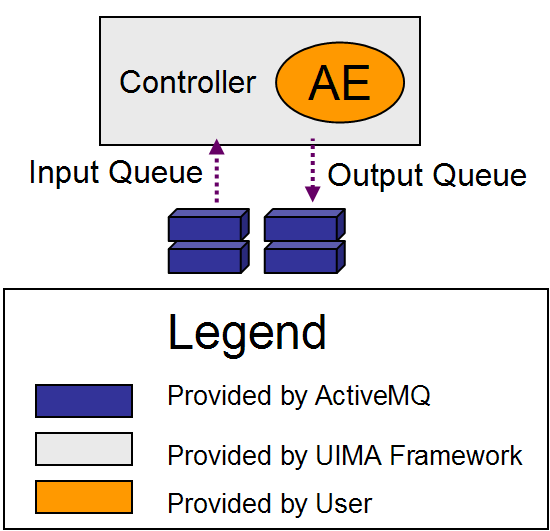
\includegraphics[width=0.5\textwidth]{uima-as-ae}
	\caption[An Analysis Engine as a service in UIMA-AS.]{An Analysis Engine as a service in \uimaas{} \cite{uimaas:documentation}.}
	\label{fig:uimaas-ae}
\end{figure}

To provide capabilities of a more complex analysis flow instead of the simple synchronous order, the user can implement what is called a \emph{Flow Controller}. An aggregate Analysis Engine can have at most one Flow Controller, that handles what \anen{} gets the \cas{} next. Usually \uima{} defaults to the \lstinline|FixedFlow| class, which executes \anens{} one after another, but more sophisticated flows can be implemented. If an aggregate Analysis Engine contains such a Flow Controller, further queues are installed. Figure~\ref{fig:uimaas-aea} shows such an advanced pipeline containing a flow controller and two delegate Analysis Engines. Submitting a \cas{} to the aggregate Analysis Engine queues it into the queue of the Flow Controller (FC). When it finishes its current computation, the Controller is faced with the decision what delegate Analysis Engine should obtain the \cas{} for processing and appends it to the corresponding queue. Notice that said queue is also provided by ActiveMQ (or any other implementation). After analysis, the \cas{} is sent back to the Flow Controller, or more specifically its output queue. It may now decide to send the processed \cas{} to another delegate \anen{} or stop processing and output it to the brokers output queue. The large amount of queue may seem excessive, but it is necessary to provide a synchronous execution of the Flow Controller and -- if configured -- the Analysis Engines.

\begin{figure}[hbt]
	\centering
	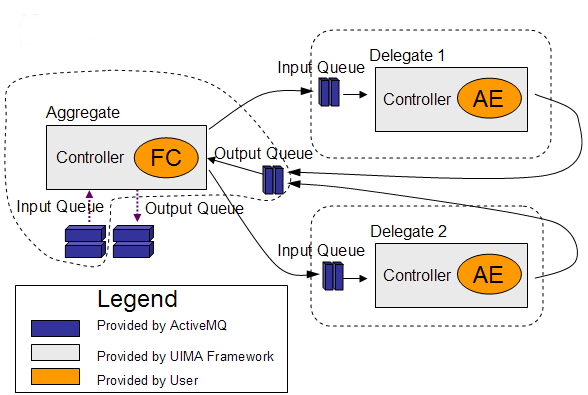
\includegraphics[width=1\textwidth]{uima-as-aea}
	\caption[An aggregate Analysis Engine as a service in UIMA-AS.]{An aggregate Analysis Engine as a service in \uimaas{} \cite{uimaas:documentation}.}
	\label{fig:uimaas-aea}
\end{figure}

Since the \cas{} object contains everything, the \sofa{}, all analysis results, the type system, and maybe even different views, it can grow quite large over the span of a complicated pipeline. This forms a problem in \uimaas{}, since the \cas{} has to be serialized for every transport inside the system, from client to broker, from broker to service, from Flow Controller to delegate Analysis Engines and the whole way back. Serialization however is a costly task and even if the underlying \nlp{} analysis is very sophisticated, serialization might not be negligible. Epstein et al. handle this problem in \cite{epstein2012making} by avoiding serialization on local instances and introducing a sparse Delta-\cas{} serialization, containing only changes in respect to an original \cas{}.

As most parts of the native \uima{} framework, \uimaas{} is configured by writing an \xml{} descriptor, containing all the necessary data for deployment. A dynamic creation of said descriptor files is currently not possible with \uimafit{}, but is provided by Leo, described in Section~\ref{ssec:leo}.

\section{Distributed Computation}
\label{sec:dist_comp}
\marginnote{Bisschen history? Eigentlich langweilig, ich erkläre hier schon extrem simple Dinge.}When handling large sets of data, a single machine may not be sufficient to solve the given task in a feasible time. In such a scenario, it would be desirable to just add more computation power to finish said task quicker. However, even if the given task permits parallelization, which is generally not obvious, distributing a problem among multiple machines, or similarly processing cores, is not trivial. For many problems a large administrative and communicative overhead aggravates the effort to parallelize.

In this section, some models for parallel and distributed computation are describes. Those concepts aim to generalize the problem of distributing a task while at the same time try not to be too restrictive in their interface. 

\subsection{MapReduce}
MapReduce is a programming model for distributed computation of large sets of data on clusters of processing cores and usually multiple machines. Google introduced the MapReduce model in 2003 and used it a few years before announcing 2014 to switch to a less restrictive framework \cite{dean2008mapreduce}.

The MapReduce process consists of three phases, \emph{Map}, \emph{Shuffle}, and \emph{Reduce}. The shuffle phase is usually provided by an implementing framework, both other phases are to be implemented by a user. Let the input data set be $C$, with identifiers $I$. More specifically this means that the following holds:

\[\forall{}c\in{}C:\exists!{}i\in{}I:i\text{ is associated with }c.\]
Furthermore let $K$ be a set of keys and $V$ a set of intermediate values. Then the map function maps the input data with the associated identifier to a list of key-value pairs:

\[\text{map}:I\times{}C \rightarrow{} (K\times{}V)^*\]
Then the \lstinline|reduce| function reduces a key and a list of all associated intermediate values to a single intermediate value:

\[\text{reduce}: K\times{}V^*\rightarrow{}K\times{}V\]

The \lstinline|reduce| function is often described with a range of just $V$, because it never changes its parameter of $K$ and just passes it through. After all value lists have been reduced to contain only a single value $v\in{}V$, they form the final output $(K\times{}V)^*$.

The canonical example for this model is the problem of counting the number of occurrences for each word in large documents or even larger corpora of documents \cite{dean2008mapreduce}. Recall that for given input documents $C$ and corresponding identifiers $I$, which might be filenames or \URL{}s, one expects a list of key-value pairs containing $k\in{}K$, an identifier for a single word (likely the word itself), and $v\in{}V$ an integer value describing the words occurrences. Figure~\ref{lst:mapreduce} shows an example implementation of said behavior. Notice that the pseudocode class \lstinline|Word| does refer to a substring containing a single word and not the unit of data.

First all documents $C$ and their identifying information $I$ are put into $|C|$ instances of the \lstinline|map| function. The results are $|C|$ lists of word-integer pairs. Notice that these intermediate results are not yet distinct. This means that several entries of even the same list might be equal if the corresponding word occurs more than once in one document. Now follows the shuffle operation, which collects intermediate results with the same key on as few machines as possible. This is a costly procedure, since data must be sent over the network. In the third phase, the reduction algorithm gets a word and a number of corresponding counting integers which it just adds and returns. Notice that -- in this example -- the first execution of the \lstinline|reduce| function will receive a word and a list of ones. This is because the \lstinline|map| function initialized each word counter with exactly one.

All intermediate results per word can now be reduced further until only one value remains, which is the final output value. Since the MapReduce model does not define an ordering on the lists given to the \lstinline|reduce| function, it must be associative and commutative to always yield the same result regardless of the inputs ordering. However, MapReduce implementations usually guarantee a fixed ordering to simplify programming the \lstinline|reduce| function.

\begin{lstlisting}[language=Java,caption={Example pseudocode implementation of the MapReduce model to count word occurrences.},label=lst:mapreduce]
List<Pair<Word, Integer>> map(Id docIdentifier, Text docText) {
	List<Pair<Word, Integer>> result = new List<>();
	for(Word w in documentText) {
		result.append((w, 1));
	}
	return result;
}

Pair<Word, Integer> reduce(Word w, List<Integer> intermediate) {
	Integer result = 0;
	for(Integer i in intermediate) {
		result += i;
	}
	return (w, result);
}

\end{lstlisting}
	
Dean and Ghemawat found in \cite{dean2008mapreduce} that many real world applications are describable in the MapReduce model. However, it is still very restrictive and has been abandoned by Google for this very reason. A popular open-source implementation of MapReduce is Apache Hadoop, or more specifically Hadoop MapReduce. It is therefore part of Apache Hadoop, a collection of utilities to handle large amount of data in computation. Apache Hadoop is popular for the \hdfs{}, a high performance distributed file system.

\subsection{Resilient Distributed Datasets}

\rdds{} provide an interface that are very similar to the native Java \lstinline|Collection|. They were initially developed in 2012 by Zaharia et al. in \cite{zaharia2012resilient} as a response to iterative algorithms being inefficient in current computing frameworks such as MapReduce.

An \rdd{} can be created by either of two ways. First, stable data collections such as native Java \lstinline|Collection| instances or a number of files in a file system can be initialized as \rdds{}. The other way of creating is a deterministic operation on an already existing \rdd{}. These operations are called \emph{transformations} by Zaharia in \cite{zaharia2012resilient}. Since \rdds{} are immutable collections, calling such a transformation on an existing \rdd{} is the only way of obtaining the wanted resulting \rdd{}.

Being immutable, \rdds{} allow to be materialized lazily. This means that the issued transformations are executed just in time, when a materialized form of the \rdd{} is necessary. This happens on actions like counting the number of objects in the \rdd{} or serializing it to a file. Before executing these transformations, an acyclic graph is built to represent the necessary transformations of computing said \rdd{}. Furthermore, \rdds{} are sliced into partitions, atomic pieces. These partitions can then be distributed among the clusters nodes and computed whenever necessary. For the distribution of said partitions, \spark{} utilizes the knowledge of the issued transformation to evaluate dependencies of resulting \rdds{} to their predecessor. This means for example, that a \lstinline|count| operation that follows a large amount of transformations does not necessarily force \spark{} to actually compute all these transformations. For example a transformation \lstinline|crossProduct| on data sets $X$ and $Y$ is guaranteed to result in a collection of size $|X|\cdot{}|Y|$. Materialization of $X\times{}Y$ is not necessary. This technique of lazy transformation provides a simple way of fault tolerance since only the \rdd{} lineage and not the complete materialized \rdd{} itself must be replicated among the different machines.

The only current implementation of \rdds{} is Apache \spark{}, introduced along with \rdds{} in 2012 \cite{zaharia2012resilient}.

\section{Docker}
Urgh, reden über Docker

\section{Related Work}
\label{sec:related}
Taking effort to scale \uima{} has been done numerous times. The most prominent result was the implementation of the question answering system Watson \cite{epstein2012making}. This approach used native \uimaas{}, although the engineers changed the \uimaas{} source code themselves. Other approaches that are trying to be generic solutions while not posing too many restrictions or being too intrusive into the native \uima{} concepts or even code, are Leo and v3NLP.

\subsection{Leo}
\label{ssec:leo}
The Leo framework was developed by \vinci{} to allow for the easy deployment of annotators in an \uimaas{} environment \cite{leo}. Since it wraps around most concepts of \uima{} and \uimaas{}, its architecture closely resembles \uimaas{}. This can be seen in Figure~\ref{fig:leo}. Given a number of instances of \lstinline|LeoAEDescriptor|, which are compatible with the native \uima{} Analysis Engine, Leo is able to automatically write an \uimaas{} deployment descriptor file and use it to deploy a \lstinline|Service| instance. This also is just a wrapper around \uimaas{} native service, which tries to register to a given broker implementation. Leo does not provide a broker implementation by its own, but depends on an existing \uimaas{} installation, which in turn provides ActiveMQ, as described further in Section~\ref{ssec:uimaas}.
\begin{figure}[hbt]
	\centering
	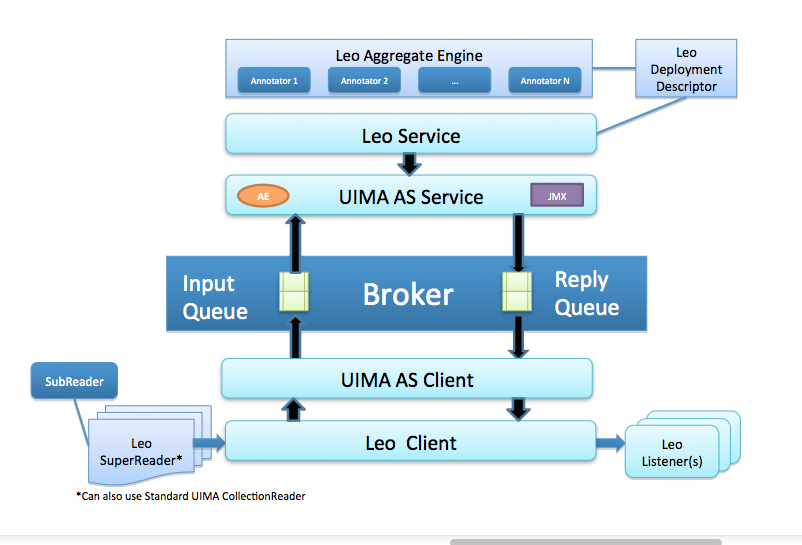
\includegraphics[width=1\textwidth]{leo}
	\caption[The Leo architecture wrapping around UIMA-AS.]{The Leo architecture wrapping around \uimaas{} \cite{leo}}
	\label{fig:leo}
\end{figure}
Given such an instance of a broker-service architecture, Leo is now able to perform requests to said broker. The Leo \lstinline|Client| class provides access to the native \uimaas{} capability of querying the services for analysis results. For this, Leo utilizes the class \lstinline|LeoCollectionReader|, which also is just a wrapper around the native \uima{} Collection Readers and can be easily converted to one and vice versa.

The Leo source code repository\footurl{https://github.com/department-of-veterans-affairs/Leo}{2018-09-14} shows that the last change was in January 2018, without providing any comments or history\footurl{https://github.com/department-of-veterans-affairs/Leo/commit/038f7d5c542fa564c2997403769943ac47638692}{2018-09-14}. This, and the fact that the project only has four contributors and no pull request as of the time of writing shows that the Leo framework project is not well-maintained.

A static code analysis with FindBugs\footurl{http://findbugs.sourceforge.net/}{2018-09-14} on the current source code\footnote{Commit 038f7d5c542fa564c2997403769943ac47638692 on 2018-09-14} shows 29 potential bugs, of which seven are rated as `scary' by FindBugs. Another code analysis tool, SonarLint\footurl{https://www.sonarlint.org/}{2018-09-14} which also checks the coding style found a total of 626 bugs, vulnerabilities and code smells. 

\subsection{v3NLP}
The framework v3NLP was first introduced in 2011 by Divita and Trietler in \cite{divita2011finding} as a successor to HITEx\footnote{Health Information Text Extraction}. Both, HITEx and v3NLP were initially built on top of the Gate framework but switched to \uima{} since. v3NLP provides capabilities to process \nlp{} tasks especially in the medical field. It is therefore heavily influenced by the context of a medical environment. It provides 34 pre-composed pipelines, all related to clinical text analysis. However, it enforces the use of the CHIR\footnote{Consortium for Healthcare Informatics Research} Common Model, which is an ontology of labels from already existing \nlp{} systems. This model is encoded in a default type system the framework is using and it can be extended at will. This is supposed to ensure interoperability between different \nlp{} components that were developed for v3NLP. Notice that this poses a restriction on the user of the framework, since they are forced to always include this type system \cite{divita2016v3nlp}. The framework also provides scaling capabilities that internally utilize the native \uimaas{} scalability.

While the v3NLP framework provides many functionalities for \nlp{} research in the medical context, it is a large project in respect to \uima{}, \uimaas{} and Leo (described in Section~\ref{ssec:leo}). All the v3NLP git repositories combined span 23.3\,GB of content and contain about 1.8\,million lines of Java code in the latest commit alone. Thus it is a heavyweight tool, which is used best in a medical environment where as many capabilities as possible are actually used.

At the time of writing, the last commit to the framework repository was on December 2017, nine months in the past. According to the v3NLP website\footurl{http://inlp.bmi.utah.edu/redmine/docs/v3nlp-framework/News.html}{2018-09-14} this is expected to be the very last commit.




%In this chapter, we will cover the basics for the necessary technologies used throughout the evaluation. All of these are concrete implementations of more general concepts and may be exchanged for similar products. However, the following products were chosen, mainly because they are Open Source\footurl{https://svn.apache.org/viewvc/uima/}{2018-02-27}\footurl{https://github.com/docker}{2018-02-27}\footurl{https://github.com/apache/hadoop}{2018-02-27}\footurl{https://github.com/apache/spark}{2018-02-27}\footurl{https://github.com/apache/kafka}{2018-02-27} but also because of their popularity and relevance in the industry.

% % !TeX root = ../Main.tex

\section{UIMA}
\uima{} is a data mining and \nlp{} framework, created in 2005 by IBM \cite{ferrucci2004uima} and maintained by Apache since 2006 \cite{uimacpe}. It is available in Java and C++ and contains various scale-out options. 
Strictly speaking, one has to differentiate between the \uima{} specification and Apache \uima{}, an open source implementation of said specification \cite{OASIS:UIMA:2009}. Since both terms are often used interchangeably, this thesis will also not differentiate between Apache \uima{} and \uima{}. Unless specified else, we will always reference the Apache \uima{} implementation.

\marginnote{Alles ein wenig wirr. Braucht rewrite. Weiß aber nicht genau wie tief in die Materie ich hier gehen muss.}
The \uima{} specification describes \nlp{} applications as a collection of (mostly) independent components. Such a component is called an \anen{} and enriches a given document by inferred information. To modularize said components, \uima{} provides the notion of a \cas{}. A \cas{} is an object containing the \sofa{}, the analysis results and the used type system.



% % !TeX root = ../Main.tex

\section{\docker{}}
\marginnote{Source?}\docker{} is a software to create and run applications in virtual environments, without the need to setup a complete virtual operating system for each application. Based on Cgroups and namespaces, \docker{} runs applications in a containerized environment.
To create a containerized application, a special markup file, called a Dockerfile has to be written by the programmer. The Dockerfile defines exactly how the applications' environment needs to look like. Listing \ref{dockerfile} shows how such a Dockerfile typically looks like. Based on an Ubuntu image, it installs Java via apt-get. Afterwards it copies the file {\em{} application.jar} into the root of the image and tells \docker{} to execute it via \lstinline[]|java -jar /app.jar -Xmx4G -Xms4G|. Having such a Dockerfile ensures reproducibility of the constructed images. After building said Dockerfile, an image is created.\marginnote{source für Registries? Öffentliches \docker{}-Registry?} This image can be serialized into a file but is usually uploaded to \docker{} repositories, called registries. 

\begin{minipage}{\textwidth}
	
\begin{lstlisting}[style=YAML,caption=A sample Dockerfile used for creating a simple Ubuntu based image to start a Java application.,label=dockerfile]
FROM	ubuntu

RUN		apt(*@-@*)get update
RUN		apt(*@-@*)get install openjdk(*@-@*)9(*@-@*)jre

COPY	./application.jar /application.jar

ENTRYPOINT ["java", "(*@-@*)jar /app.jar", "(*@-@*)Xmx4G", "(*@-@*)Xms4G"]
\end{lstlisting}

\end{minipage}

\marginnote{SOUUUURCE!!}If published through a registry, \docker{} automatically downloads images on demand. Since the application as well as the whole environment necessary to run it lie within the image, it can be executed. \docker{} creates a container, a virtual environment based on the given image, \marginnote{Zweimal within? Thesaurus lässt grüßen.}and runs the application within. Containers are usually not aware of each other, thus the same application can be started multiple times, just by starting more containers. \marginnote{An den Haaren herbeigezogen.}This modular view on containers will play a fundamental role on scaling.
% % !TeX root = ../Main.tex

\section{Hadoop}
\marginnote{Sauce!}\hadoop{} is an open-source framework for computation and storage, distributed over an \marginnote{almost?}(almost) arbitrary number of machines. It contains the \hdfs{}, a distributed file system built for high throughput and reliability, and specifically designed to run on commodity hardware. These properties allow for large clusters of relatively cheap hardware.

\hadoop{} also provides an API for distributed computing, named Hadoop MapReduce, based on the MapReduce algorithm by Dean and Ghemawat in \cite{dean2008mapreduce}. In this algorithm the underlying transformation of data is abstracted into two general steps, Map and Reduce. With $K,L,V,W$ being sets the Map function implements 
\[\mathtt{Map}: K\times{}V\to{}(L\times{}W)^*\]
Thus it maps a key-value pair to a list of key-value pairs of arbitrary length \cite{wiki:mapreduce}. The resulting list of key-value pairs acts as intermediate values. The Reduce function aggregates those intermediate values with
\[\mathtt{Reduce}: L\times{}W^*\to{}\] huh...
The programmer in question needs to understand this concept and divide their code into those two steps.
% \section{Spark}
% \section{Kafka}

\chapter{Implementation}
\label{ch:implementation}
In this chapter we will first discuss the choice of \spark{} as a distribution technology. Afterwards the framework implementation details will be documented with a special focus on data distribution, namely Serialization and Compression.
\section{Technologies}


Erkläre die Entscheidung warum auf Spark gesetzt wurde als Distributionsframework. Das möglicherweise mit Kruchten 4+1 (\url{https://de.wikipedia.org/wiki/4\%2B1_Sichtenmodell})  aufhübschen.

Ich sollte auch ein wenig mit den generischen Ansätzen Compression \& Serialization angeben. War schließlich nicht trivial die scheiße zu entwickeln.

Timm schlägt ein Schichtendiagramm vor, das zeigt wo ich zwischen UIMA und Spark stehe. Klingt gut, aber auch recht kompliziert in der Umsetzung. Ich denke das werde ich als letztes machen.

Ich denke aus diesen Bildern kann sich recht kanonisch eine Gliederung für das Kapitel entwickeln. Hier mal eine Liste von Abbildungen, die ich mir bisher vorstelle

Framework schematisch in Netzwerksicht (Also welchen Weg Dokumente so in meinem FW gehen)



\section{Implementation}


\section{Data Distribution}
Since all the input data, in form of documents, and output data, in form of analysis results, must be transmitted over a network, be it virtual or real, the serialization of larger Java objects play a role in performance. Since both, the input and the output, are stored inside a \cas{} object it suffices to find a suitable serialization algorithm for those. However, finding an optimal algorithm is not trivial and usually even depends on the input data. Larger documents produce larger \cas{}, which in turn need a longer time to be deployed to the corresponding \spark{} workers. However, small documents still are no guarantee for small \cas{} sizes, since analysis results can be of arbitrary size and number, depending on the \uima{} pipeline. 

Furthermore it can be useful to compress serialized data, depending on the network setup and the serialization algorithm. Most native \uima{} serializations produce \xml{} files, which are very verbose and well compressible. Compression algorithms specifically designed for \xml{} files achieve packing ratios of up to 80\,\% \cite{girardot2005system,min2003xpress,sakr2009xml}. However, such algorithms often come at the price of a relatively high runtime. This is especially undesirable if the transmitted data is small or the serialization sparse and the expected compression ratio is low.

Since an optimal choice for both, serialization and compression, is not possible for the general case the framework exposes two interfaces, namely \lstinline|CasSerialization| and \lstinline|CompressionAlgorithm|.
\subsection{Serialization}
In \cite{epstein2012making} Epstein et al. explain how serialization of \cas{} was an important bottleneck and a problem to solve. They configured \uimaas{} in several ways to serialize only the parts of the \cas{} object that are needed for further analysis. Obviously this can not be done in the general case when the underlying analysis algorithms are unknown, which is why the framework takes an instance of \lstinline|CasSerialization| as an optional parameter.

An instance of said interface implements two methods with the signatures shown in Listing~\ref{lst:casserialization}..
\begin{lstlisting}[language=Java,caption={CasSerialization method signatures},label=lst:casserialization]
public byte[] serialize(CAS cas);
public CAS deserialize(byte[] data, CAS cas);
\end{lstlisting}

While the signature of the \lstinline|serialize| method is intuitive, this does not immediately apply to the \lstinline|deserialize| function. Here, a previously created \cas{} object is given as a parameter for two reasons. First, \uima{} allows for the configuration of a custom \lstinline|CasInitializer|, which can alter the \cas{} object immediately after creation. Although the usage of \lstinline|CasInitializers| has been deprecated since at least 2006, it is still a feature of \uima{} and must therefore be taken care of \cite{uimacpe}. By creating a new \cas{} on the target \jvm{}, the framework first executes the \lstinline|CasInitializers| and then passes the resulting \cas{} to the \lstinline|deserialize| function. The second reasons for this additional parameter is to pass the current \uima{} type system. The serialized data might include annotations of types that are unknown to the native \uima{} type system and therefore must be defined before deserialization. Although a parameter \lstinline|TypeSystem| would have been sufficed, the first reason implies the requirement of a complete \cas{} parameter. Since the created \cas{} already includes the full type system description, available by \lstinline|cas.getTypeSystem()|, the framework abstains from passing another parameter to the \lstinline|deserialize| method. If \lstinline|CasInitializer|s get removed from \uima{}, this might be a feasible change in the future.

The framework already ships with two implementations of the \lstinline|CasSerialization| interface, namely \lstinline|XmiCasSerialization| and \lstinline|UimaCasSerialization|. The \lstinline|XmiCasSerialization| creates complete \xmi{} files, containing the \sofa{}, all analysis results and even the used type system description. To accomplish this, it uses the \uima{} \lstinline|XmiCasSerializer| class. Thus, the \lstinline|XmiCasSerialization| implementation of \lstinline|CasSerialization| acts as a mere wrapper. The second serialization algorithm \lstinline|UimaCasSerialization| also just wraps around the native \uima{} class \lstinline|Serializer|, which is the same serialization algorithm \uimaas{} uses to distribute and retrieve \cas{} objects.

\subsection{Compression}
Since the compression results are very dependent on the use case, data size and serialization algorithm, the framework provides the user with a \lstinline|CompressionAlgorithm| interface. An implementation of said interface exposes two methods with signatures as shown in Listing~\ref{lst:cascompression}.
\begin{lstlisting}[language=Java,caption={CompressionAlgorithm method signatures},label=lst:cascompression]
public byte[] compress(final byte[] input);
public byte[] decompress(final byte[] input);
\end{lstlisting}
Completely abstracted from any \uima{} concept, this interface simply expects two functions, \lstinline|compress| and \lstinline|uncompress| to behave such that for every input \lstinline|byte[] X| holds that \lstinline|X = decompress(compress(X))|. While this is the only technical requirement for this interface, it is usually desired to have \lstinline+|X| > |compress(X)|+. Since both methods act \uima{} unaware, reducing the object size by omitting parts of the \cas{} is not possible without deserializing the \cas{} first, a step that is defined in the \lstinline|CasSerialization| interface and not accessible from this context. 

The framework ships with two implementations of the \lstinline|CompressionAlgorithm| interface. If defaults to the \lstinline|NoCompression| class, simply implementing the identity with \lstinline|X = compress(X)|, effectively disabling any kind of compression. This is useful if network delay is negligible, especially in virtual networks inside a single machine. A compression algorithm would need computation time to process all transmitted \cas{}, while saving only a minimum of transfer time. Secondly, the class \lstinline|ZLib| implements the DEFLATE compression, which is a general purpose lossless compression algorithm, commonly used in ZIP files.

		% Hauptteil, Lösungen von Problemen, Implementierungsdetail(?)
\chapter{Evaluation}
\label{ch:evaluation}
In the following sections, the framework introduced in Chapter~\ref{ch:implementation} will be compared to existing \uima{} distribution approaches. For this reason, a sophisticated evaluation architecture was deployed on a virtual network, which is described in Section~\ref{sec:setup}. The comparison will follow along the metrics given in Section~\ref{sec:requirements}~`\nameref{sec:requirements}'.


\section{Setup}
\label{sec:setup}

Setting up a testing and benchmarking environment for the framework given in Chapter~\ref{ch:implementation} and \uimaas{} is not trivial when accounting for comparability. This is because the given framework and \uimaas{} function fundamentally different from each other. The following descriptions for \docker{} architectures suggest a highly similar setup, but even the initialization of both systems differ in terms of concept. While the actual analysis code inside the aggregate \anen{} is provided at the \uimaas{} services inherently, this does not hold for a \spark{} cluster. Such a \spark{} cluster waits for tasks until one arrives and orders it to execute code according to a JAR file, whose \URL{} is given in a parameter. However, the same cluster can work on other problems as well, without reconfiguration and reinitialization. Different tasks can even be processed in parallel, since the \spark{} is not just usable by the framework's \api{}.

This concept is fundamentally different from \uimaas{}, where a service is bound to exactly one aggregate Analysis Engine and therefore one pipeline. If another \nlp{} algorithm has to be processed, another \uimaas{} service must be instantiated and registered to the broker, at another queue name. While the old services are still up, system resources for those can not be reallocated and idle until a \cas{} object for exactly this \anen{} is sent to the broker. 

These two concepts both have their advantages and disadvantages. The way \spark{} allocates resources for tasks makes it more flexible to use. Different pipelines can easily be processed without making changes to the computation cluster. A cluster of \uimaas{} services would need heavy reconfiguration for such a case. However, since \uimaas{} services do not discard their resources after finishing the current task, a pipeline does not need to be reinitialized if another \cas{} should be analyzed. Since \nlp{} algorithms commonly depend on large dictionaries or language models, this saves on loading time and especially disk I/O. A \spark{} cluster would immediately forget the context of the current pipeline and would have to reinitialize it.

This also comes into play when evaluating the running time of both concepts. Given a more sophisticated pipeline and a ready-to-use \spark{} cluster on the one hand and a number of \uimaas{} instances on the other, the pipelines in the \uimaas{} services would have already been initialized, while the pipelines in the \spark{} architecture are initialized on-the-fly. This holds not true for \anens{} that load their resources lazily. However, no such assumption can be made in general.

To evaluate both frameworks, and the single-threaded approach to get a sense of the administrative workload, a cluster of multiple computers was needed. To simulate a network of machines, \docker{} was chosen as a virtualization concept for multiple reasons. First, \docker{}s resource footprint is way smaller than one of a virtual machine, therefore more resources can be allocated for the actual benchmark. Secondly, a docker image is completely reproducible. While this can also be achieved with configuration management tools like Chef\footurl{https://www.chef.io/chef/}{2018-09-16}, Puppet\footurl{https://puppet.com/de}{2018-09-16} or Ansible\footurl{https://www.ansible.com/}{2018-09-16}, defining a Dockerfile allows for easy reproduction and configuration. 

Notice that network transport delay between the various components are trivial in a simulated network without any artificial delay. For this reason, compression was disabled for the framework presented in this thesis.

\subsection{Hard- and Software}
The hardware setup consisted of one Intel Xeon E5-1650 with 6x2.6\,GHz with 128\,GB DDR4 memory clocked at 2400\,MHz. The host operating system was an Ubuntu~16.04~LTS with \docker{}~17.12.1-ce installed. For executing the \jvm{}s, openJDK \docker{} images were used, containing the openJDK~8u181. \uima{} and \uimaas{} were used in version 2.10.2 and the \dkpro{} Analysis Engines are taken from the repository version 1.8.0.

\subsection{Apache Spark}
\label{ssec:spark}
In Figure~\ref{fig:arch-spark}, one can see the \docker{} architecture used in the evaluation. A custom created image for \spark{} was used for both, the master and the worker nodes. This image is based on OpenJDK and will be available as described in Section~\ref{sec:availability}. The \spark{} worker nodes can be scaled at will by a simple \docker{} parameter. Both containers, \emph{jar-provider} and \emph{document-provider} are  instances of nginx\footurl{https://www.nginx.com/}{2018-09-16} HTTP servers. The document provider simply provides access to the complete corpus of documents via ordinary HTTP GET requests. These documents could have also been simply copied into the \emph{submitter} image, however an HTTP provider server for the document corpus was chosen to equalize I/O delay, both \uimaas{} and \spark{} would have. This approach is also easily modifiable since the documents provided by the nginx server are a volume, pointing to a persistent folder inside the host file system.
\begin{figure}[tbh]
	\centering
	\input{img/docker-architecture-spark.pdf_tex}
	\caption[The evaluation architecture with Spark inside a Docker environment.]{The evaluation architecture with \spark{} inside a \docker{} environment.}
	\label{fig:arch-spark}
\end{figure}
Similarly, the jar-provider provides the needed JAR files for \spark{} worker nodes. As described above, a \spark{} cluster is a general computation cluster and not pipeline-specific. Thus, to execute code of an Analysis Engine, the corresponding JAR file must be provided to the whole cluster. While this can also be achieved by mounting a persistent folder inside each worker and the master node, it seemed a cleaner solution to expose the JAR file by another nginx HTTP server. This is closer to real world applications, because a JAR file will most likely not first be copied to each worker node's file system before executing, especially since it is not trivial to predict which workers are actually processing the given tasks and at what time. In this architecture, any worker can access the JAR file at any point of its lifetime.

The submitter container is also an instance of the \spark{} image described above, but only issues the initial command to the cluster. \spark{} works in one of two modes. First, the standalone mode would let the submitter container also download the JAR file and execute the code until a Java command issues the cluster to work on some tasks in a distributed manner. In cluster mode, a worker node would be allocated by the clusters master to execute the Java code. When a Java command orders \spark{} to parallelize some work, more resources are allocated for said tasks. However, the initial worker node would be unavailable for this phase. Since the architecture is more comparable to the \uimaas{} architecture in the standalone mode, it was chosen for the evaluation.
\subsection{UIMA-AS}
The \docker{} architecture in the evaluation setup for \uimaas{} is very similar to the one for \spark{}. In Figure~\ref{fig:arch-uimaas}, the deployment composition is shown. For the \uimaas{} services, the underlying ApacheMQ broker and the submitter container, an \uimaas{} \docker{} image was composed. As with the \spark{} image described in Section~\ref{ssec:spark}, it is based on an OpenJDK image and will be available to the public according to Section~\ref{sec:availability}.
\begin{figure}[htb]
	\centering
	\input{img/docker-architecture-uimaas.pdf_tex}
	\caption[The evaluation architecture with UIMA-AS inside a Docker environment.]{The evaluation architecture with \uimaas{} inside a \docker{} environment.}
	\label{fig:arch-uimaas}
\end{figure}
First, the \uimaas{} services register themselves at the given broker instance. At the same time the services initialize their corresponding pipeline. This happens in contrast to \spark{}, where the given cluster is completely \uima{} agnostic and initializes the pipelines when they are needed.

In the same way as in Section~\ref{ssec:spark}, the submitter reads the documents per HTTP from the document-provider, which is an instance of the identical image used in the \spark{} evaluation. Notice that even the logic of reading the corpus is identical, since it is wrapped inside a \lstinline|CollectionReader|, which produces \cas{} object that can be processed further. The \cas{} are then sent to the broker and distributed among the services. An important distinction to make is that in the \uimaas{} concept the \cas{} object must return to the submitter. In contrast, the concept of the framework built on top of spark does allow the collection of the resulting \cas{}, but discourages it, since it may be a bottleneck on large corpora or large pipelines providing many analysis results.

\subsection{Analysis Engines}
\label{ssec:pipelines}
Since the performance is most likely very dependent on the actual analysis to run, or more specifically the given pipeline, three different pipelines were used to compare \uimaas{} and \spark{}:
\begin{itemize}
	\item{}Parsing
	\begin{enumerate}
		\item{}\emph{Language Setter}: Sets the \cas{} language to English. 
		\item{}\emph{Stanford Segmenter \cite{manning-EtAl:2014:P14-5}}: Segments the text into tokens for further processing.
		\item{}\emph{Stanford PoS Tagger \cite{manning-EtAl:2014:P14-5}}: Finds the parts-of-speech for all identified tokens \cite{toutanova2003feature}.
		\item{}\emph{Malt Parser\cite{Nivre05maltparser:a}}: Locates the grammatical components of sentences.
	\end{enumerate}
	\item{}Mixed Named Entity Recognition
	\begin{enumerate}
		\item{}\emph{Language Setter}: Sets the \cas{} language to English. 
		\item{}\emph{OpenNLP Segmenter \cite{opennlp}}: Segments the text into tokens for further processing.
		\item{}\emph{Mate PoS Tagger \cite{bohnet2010very}}: Finds the parts-of-speech for all identified tokens.
		\item{}\emph{ClearNLP Lemmatizer \cite{manning-EtAl:2014:P14-5}}: Generates the base forms for all identified tokens.
		\item{}\emph{Berkeley Parser\cite{petrov2006learning,petrov2007improved}}: Locates the grammatical components of sentences.
		\item{}\emph{Stanford Named Entity Recognizer \cite{manning-EtAl:2014:P14-5}}: Finds occurrences of the entities `Person', `Location', `Organization' and `Misc' and numerical entities.
	\end{enumerate}
	\item{}OpenNLP Named Entity Recognition
	\begin{enumerate}
		\item{}\emph{Language Setter}: Sets the \cas{} language to English. 
		\item{}\emph{OpenNLP Segmenter \cite{opennlp}}: Segments the text into tokens for further processing.
		\item{}\emph{Mate Lemmatizer \cite{bohnet2010very}}: Generates the base forms for all identified tokens.
		\item{}\emph{OpenNLP PoS Tagger \cite{opennlp}}: Finds the parts-of-speech for all identified tokens.
		\item{}\emph{OpenNLP Named Entity Recognizer \cite{opennlp}}: Finds occurrences of entities according to a pre-defined model.
		
	\end{enumerate}
	
\end{itemize}
All the given Analysis Engines (except for the Language Setter) are provided by the \dkpro{} repository via the build tool maven. 

\subsection{Document Corpus}
The evaluation was used to analyze a corpus of 3036 text files, taken from the larger dataset of the project Gutenberg\footurl{http://www.gutenberg.org/}{2018-09-16} \cite{lahiri:2014:SRW}. This subset was cleaned from metadata, license information and transcribers notes and were therefore seen as more realistic input data than books containing such artifacts. Furthermore books were chosen as analysis items, because they contain large amount of natural language and may revolve around very different domains. This can be important for the performance of algorithms that solve specific \nlp{} tasks, for example Named Entity Recognition. 

For the analysis, the corpus was partitioned into three slices of equal cardinality according to file size. The smallest third of all files are files up to a size of 193\,kB. A file is in the middle partition, if it is larger than 193~,kB, but also at most 459\,kB. The largest file was about 9~,MB, therefore an upper limit for even the biggest files is 10000\,kB.
\section{Results}

In the following sections the results of said evaluation are described.

\subsection{CPU Usage}
Evaluating the CPU usage actually turned out to be surprisingly simple. Both, \uimaas{} and the framework implementation of Chapter~\ref{ch:implementation} used all the available processor resources when needed. This is largely due to the fact that every (virtual) machine that represented worker nodes or services respectively, got exactly one processor core. Since no waiting time or disk I/O was necessary to process the pipelines given in Section~\ref{ssec:pipelines}, nothing stopped any of both frameworks utilizing the maximum processor time available.

Both frameworks also acted the same when idling, taking no measurable processor time. This may be due to the blocking system call \lstinline|accept|\footurl{http://man7.org/linux/man-pages/man2/accept.2.html}{2018-09-18} that does not introduce any CPU overhead.
\subsection{RAM Usage}
The usage of RAM was mostly neglected on the evaluation. This is because of two reasons: First, the actually used RAM is highly dependent on the underlying algorithm. It showed that both, \uimaas{} and \spark{} had negligible overhead relative to the memory actually needed by the Analysis Engines. Even simple \anens{} load models or static resources to process the given \cas{} and if the necessary resources, including the input \cas{} and the resulting analysis objects can not fit into the provided memory, no approach that includes \uima{} is feasible.

The second point why RAM is neglected in this evaluation is the availability of it. The final evaluation run allocated 10\,GB of memory to each processing container. This was an arbitrary choice, as 4\,GB would have also sufficed, which is a low amount of memory in a cluster computation environment and one could argue that a sufficient amount of memory will always be available. Notice that an algorithm does not generally run faster with more available memory. It rather avoids swapping, using the hard drive to extend the available memory, making the actual usage of RAM a binary question: Is there enough to completely avoid swapping? In favor of focusing the other metrics, this question was answered `yes' for this evaluation.

\subsection{Document Throughput}
Analyzing the number of documents that get processed per second shows how fast the different frameworks process the documents without taking account for the differing document sizes. As one can see in Figure~\ref{fig:result:throughput}, the throughput for the single-threaded \uima{} and the \uimaas{} implementation are similar, which seems confusing at first but will be explained in a more detailed view later. It is intuitive that larger document sizes produce smaller results at document throughput. However, \spark{} achieves better results when given more work load in this figure.
\begin{figure}[!htb]
	\centering
	\resizebox{1.\linewidth}{!}{\small\input{img/document_throughput_to_size.pdf_tex}}
	\caption[The document throughput of each framework in the three size categories.]{The document throughput of each framework in the three size categories.}
	\label{fig:result:throughput}
\end{figure}
This is due to the fact that the Analysis Engine initialization is contained in the deployment of \uimaas{}, but also in the processing time of the \spark{} approach. As discussed earlier, this is a fundamental difference between both frameworks and can not simply be omitted, since initialization is often a costly part of an \anen{} life cycle. However, having larger corpora of data that can be processed at once, without reinitializing the pipelines, this overhead becomes less significant and the document throughput per second rises. This can be seen as a head start for both, the single-threaded approach and \uimaas{}. This head start is sacrificed by \spark{} in order to provide a more flexible interface as explained in Section~\ref{sec:setup}.
\begin{figure}[htb]
	\centering
	\resizebox{1.\linewidth}{!}{\small\input{img/document_throughput_detailed.pdf_tex}}
	\caption{The document throughput of each framework in the three size categories, detailed.}
	\label{fig:result:throughput_det}
\end{figure}
As for the similarity between the single-threaded approach and \uimaas{}, one can see in Figure~\ref{fig:result:throughput_det} that both perform indeed differently, depending on the size of the corpus. Here, the size of the corpus is measured in number of files in the corresponding size category. The single-threaded instance of a native \uima{} pipeline remains stagnant, which is to expect since no increase in administration overhead is necessary to process more data. However, with increasing corpus size, \uimaas{} performs better, since the broker can actually utilize the additional resources.

One can also see an increase in the performance of \spark{}, but it is rather slow compared to \uimaas{}. Only on large corpora of big documents, \spark{} achieves better results than both competitors for reasons described above.

\subsection{Byte Throughput}
Measuring the throughput in terms of bytes per second is a little more complicated than the metric before, because there are different ways to interpret the amount of bytes a process is associated with. Since pipelines usually make annotations and therefore add something to the \cas{} object, the output size is generally not equal to the input size. However, taking compression and serialization into account, the final output size is not equal to the size transmitted between the different components, at least in the case of \spark{} and \uimaas{}.

Thus, two slightly different measures are shown in Figure~\ref{fig:result:throughput_bytes} and Figure~\ref{fig:result:throughput_bytes_after}. Figure~\ref{fig:result:throughput_bytes} shows the number of bytes \emph{before} processing the document and Figure~\ref{fig:result:throughput_bytes_after} shows the same, but calculated with the amount of bytes the \cas{} object holds \emph{after} analysis. Recall that a \cas{} object holds all necessary data, the \sofa{} and all analysis results. Thus it is input and output at the same time, serving well for a size indicator.

In the first figure (Figure~\ref{ref:result:throughput_bytes}), one can see that the single-threaded implementation again stagnates as expected. Since different document sizes are processed exactly the same, the throughput in bytes per second does not change with increasing input sizes. This however, does not hold for \uimaas{} and \spark{}. One can see that \uimaas{} profits from having larger document sizes, most likely because not all available resources could be utilized on the smaller instances. Once every resource is used near optimally, the performance of \uimaas{} also stagnates in terms of byte throughput. Notice that this is to be expected by \emph{any} framework with a constant amount of computation resources.
\begin{figure}[htb]
	\centering
	\resizebox{1.\linewidth}{!}{\small\input{img/byte_throughput_to_size.pdf_tex}}
	\caption{The byte throughput of each framework in the three size categories, measured in bytes before the analysis.}
	\label{fig:result:throughput_bytes}
\end{figure}
\spark{} first drops to a lower performance when increasing the document size and then rises above both other approaches. The first drop is again most likely due to the initialization of Analysis Engines. For the same reason \uimaas{} performs better at medium input sizes, \spark{} starts to actually use all available resources, triggering the pipeline initialization as often as worker nodes in the \spark{} clusters are. Since the larger documents are bigger by an order of magnitude, this initialization again becomes more and more insignificant.
\begin{figure}[htb]
	\centering
	\resizebox{1.\linewidth}{!}{\small\input{img/byte_throughput_to_size_after.pdf_tex}}
	\caption{The byte throughput of each framework in the three size categories, measured in bytes after the analysis.}
	\label{fig:result:throughput_bytes_after}
\end{figure}
Figure~\ref{fig:result:throughput_bytes_after} shows a similar trend. However, here all algorithms perform worse at smaller input data. This might be because the \cas{} objects do not grow linearly in size after the analysis by the given three pipelines, since fewer annotation types must be shipped within the type system. Another reason is the overhead \uima{} provides itself, making processing of small data more inefficient. However, since \uima{} is the underlying framework for all three approaches, every one of them suffers the consequences.




\subsection{Maintainability}
Given a working \spark{} cluster and the corresponding \uimaas{} service collection, changing the underlying Analysis Engine varies from each of the three evaluated approaches in multiple aspects. 

A single-threaded native \uima{} instance is exactly as complicated to change as the new Analysis Engine is easy to configure. \anens{} can be arbitrarily complex and thus, their configuration options may as well. Since each approach has to deal with this, it can be ignored while comparing all three implementations. This, however, leaves the single-threaded approach to be trivial to reconfigure. One can observe this in real life applications and stems from the very generic interface the \lstinline|AnalysisEngine| class implements.

Changing \anens{} inside an \uimaas{} environment is substantially harder. Here, all services that serve the specific broker endpoint which is associated with the pipeline, must be shut down and redeployed. This can be automated with tools like \docker{}, posing other restrictions on log persistence and adding another layer of complexity to the deployment logic. Notice that, without extra tooling such as \docker{}, each service must be shut down separately. There is no centralized command interface.

Switching \anens{} in a \spark{} environment is exactly as easy as the single-threaded approach, since \spark{} is \uima{} agnostic. At the moment code gets executed that demands the use of a newer version of the \anen{}, \spark{} will pull the modified pipeline code and therefore process the given \cas{} objects within the new \anen{} version. Notice that no changes on the cluster must be made and changing the underlying Analysis Engine is possible by only modifying the code in constant time in respect to the cluster size.
\subsection{Implementability}
Since each of the three evaluated implementations, utilizing \spark{}, \uimaas{} or just a single-threaded native \uima{} pipeline requires knowledge about the \uima{} environment, the single-threaded approach is objectively the easiest to implement. Taking sufficient knowledge of \uima{} as granted, the single-threaded approach does not require any more expertise and is therefore trivial. This is not the case with \uimaas{} and the framework presented in Chapter~\ref{ch:implementation}.

\uimaas{} relies heavily on \xml{} files for deployment configuration, most of which must be edited manually. This is an error-prone and tedious task when done by hand. The framework Leo, that builds on top of \uimaas{} helps with this by creating \xml{} descriptor files automatically. This however, requires the injection of the Leo framework, another dependency with possible errors which also increasing the size of the final code file. Having dealt with \xml{} descriptor files and the distribution of those, other obstacles occur. Neither log files for debugging purposes nor configuration options of deployed pipeline services are available from outside the service. To make changes to a deployed pipeline, all instances of said \anen{} must be stopped and reinitialized. Log files must be collected by hand, a custom script or by a third party tool. This is opposed to the framework built on top of \spark{}.

Although the framework requires knowledge about the configuration of a given \spark{} cluster, this has to be done only once. While \uimaas{} server instances need to be redeployed whenever a new project starts or changes on \anens{} occur, a \spark{} cluster must be set up once and can then be used indefinitely for different projects and especially distinct \anens{}. In an industry environment, a company wide \spark{} cluster would be imaginable. In such a scenario, configuration of the \spark{} cluster would be done once for the whole company. Thus having knowledge about \spark{} is only partially a requirement, depending on the surrounding environment. Having a running and configured instance of a \spark{} cluster at hand, the execution of the framework becomes trivial as well. Analysis Engines can be changed at will, since \spark{} is completely \uima{} agnostic. Log files are available by either configuring a proper log folder in the initial \spark{} options or by navigating to the \spark{} master node with any browser.
\subsection{Code Quality}
While strictly speaking not a metric measured in the evaluation, code quality is an important factor when deciding upon a scaling framework for \uima{}. Since the framework's code was optimized according to both static code analyzers FindBugs and SonarLint, it seems unfair to compare their feedback on the framework presented in this thesis with their results on analyzing alternatives like \uimaas{} or Leo. However, it is still a good indicator of code robustness.

While Leo was found to have 29 potential bugs according to FindBugs, and 626 bugs, vulnerabilities and code smells found by SonarLint, \uimaas{} results are way larger. With 3854 bad code artifacts identified by SonarLint and 42 potential bugs shown by FindBugs, its code robustness is debatable. This is especially important on larger projects in a setting where frequent updates are usually not possible, for example in a production environment.

This metric has to be taken with care. As described above, the framework presented in Chapter~\ref{ch:implementation} was specifically designed to output as few findings of both static code analyzers as possible. Also, both analyzers were used with the default configuration, which is usually sensible. However, if one of both, Leo and \uimaas{} would have been programmed with a different set of FindBugs and SonarLint configuration options in mind, many false positives would be expected.

Both, FindBugs and SonarLint do not find any potential bugs or vulnerabilities in the framework's code. Also the Java compiler used for compiling the framework showed no warnings.

			% Evaluation (Geschwindigkeit, Speicher etc.)
\chapter{Summary}

Hier ist ein wunderhübscher Ort um nochmal alles zusammenzufassen. Daher hat dieser Ort auch jene Überschrift bekommmen :3

\section{Limitations}
Eventuell sogar schon in die Implementierung?

\section{Conclusion}

Das hängt ein wenig von den Ergebnissen ab. Ich hoffe auf sowas wie "Ich bin der tollste, UIMA-AS ist Dreck". Das spiegeln die Daten zwar nicht ganz wieder, aber hey :D

\section{Outlook}

Spark-Funktionalitäten können noch in das Framework implementiert werden (sogar extrem leicht, da der return value ein Spark-Objekt ist). Weiterhin ist es natürlich Usern überlassen ob weitere Serializations und Compressions implementiert werden.			% Zusammenfassung / Fazit


\newpage{}
\pagenumbering{Roman}
\setcounter{page}{1}
% Glossary obv.
\printnoidxglossary[sort=letter]
% Bibliography obv.
\bibliography{bibliography}

% Eidesstattliche Erklärung des Selbstständigen Verfassens
\pagebreak
\section*{Eidesstattliche Erkl\"arung}
Hiermit versichere ich, Simon Gehring, dass ich die vorliegende Masterarbeit selbstst\"andig verfasst und keine anderen als die angegebenen Quellen und Hilfsmittel benutzt habe. Die Stellen meiner Arbeit, die dem Wortlaut oder dem Sinne nach anderen Werken und Quellen, einschlie\ss{}lich Quellen aus dem Internet, entnommen sind, habe ich in jedem Fall unter Angabe der Quelle deutlich als Entlehnung kenntlich gemacht. Dasselbe gilt sinngem\"a\ss{} f\"ur Tabellen, Karten und Abbildungen.

\vspace*{2cm}
Unterschrift: \hrulefill

\hspace*{0mm}\phantom{Unterschrift: }Simon Gehring, Student

\hspace*{0mm}\phantom{Unterschrift: }Universit\"at Bonn

  
\end{document}
